\documentclass{if-beamer}

\usepackage{pgf}
\usepackage{pgfplots}
\usepackage{amsmath}


\usepgfplotslibrary{fillbetween}

\usepackage{amssymb}
\usepackage{pifont}
\usepackage{tikz}
\usetikzlibrary{automata, positioning, arrows}


%\newcommand{\xmark}{\ding{55}}%
%\newcommand{\cmark}{\ding{51}}
\newcommand{\sep}{Explore, then plan}
\newcommand{\tog}{Simultaneous}
\newcommand{\bia}{Simult.\ biased}




% --------------------------------------------------- %
%                  Presentation info	              %
% --------------------------------------------------- %
%\title[An anytime algorithm for reachability in uncountable MDPs]{An anytime algorithm for reachability in uncountable MDPs}
%\subtitle{dsh}
%\author{Kush Grover}

\title[Robot Motion Planning]{Robot Motion Planning}
%\author{\authorblockN{Kush Grover\authorrefmark{1},
%		Fernando S. Barbosa\authorrefmark{2},
%		Jana Tumova\authorrefmark{2} and
%		Jan K\v ret\'insk\'y\authorrefmark{1}}
%	\authorblockA{\authorrefmark{1}Technical University of Munich, Germany.\\ Emails: \{grover, jan.kretinsky\}@in.tum.de}
%	\authorblockA{\authorrefmark{2}KTH Royal Institute of Technology, Stockholm, Sweden.\\ Emails: \{fdsb, tumova\}@kth.se}
%}

\author{K. Grover, F. Barbosa, J. T\r{u}mov\'a, J. K\v{r}et\'{i}nsk\'{y}}
\logo{
	
\includegraphics[scale=0.0065]{figures/tum-logo.png}
}

\institute[]{
	Technical University of Munich, KTH Royal Institute of Technology
}


% \subject{Presentation subject} % metadata

\graphicspath{{figures/}}
% --------------------------------------------------- %
%                    Title + Schedule                 %
% --------------------------------------------------- %

\begin{document}

\begin{frame}
  \titlepage
\end{frame}

\begin{frame}{Outline}
  \tableofcontents
\end{frame}

\arrayrulecolor{tableColor1}
% --------------------------------------------------- %
%                      Presentation                   %
% --------------------------------------------------- %


\section{Motion Planning Problem}

\begin{frame}
	\frametitle{Motion Planning Problem}
	\begin{center}
		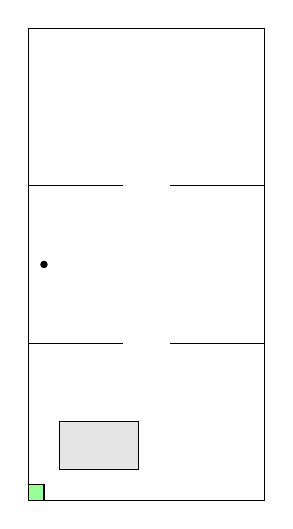
\begin{tikzpicture}
		\filldraw[fill = green!40!white, draw = black] (0, 0) rectangle (0.2, 0.2);
		\filldraw[fill = black!10!white, draw = black] (0.4, 0.4) rectangle (1.4, 1);
		\draw (0, 0) -- (3, 0) -- (3, 6) -- (0, 6) -- (0, 0);
		\draw (0, 2) -- (1.2, 2) (1.8, 2) -- (3, 2);
		\draw (0, 4) -- (1.2, 4) (1.8, 4) -- (3, 4);
		\filldraw[black] (0.2, 3) circle (0.4mm);
		\end{tikzpicture}
	\end{center}
\end{frame}

\begin{frame}
	\frametitle{RRT/RRG}
	\begin{center}
		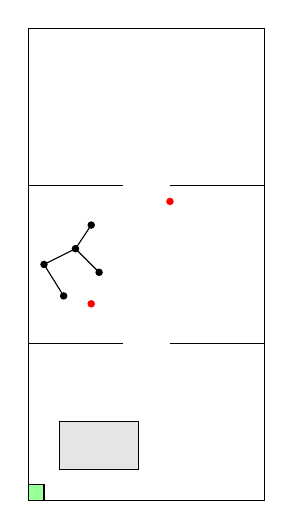
\begin{tikzpicture}
		\onslide<0->{
			\filldraw[fill = green!40!white, draw = black] (0, 0) rectangle (0.2, 0.2);
			\filldraw[fill = black!10!white, draw = black] (0.4, 0.4) rectangle (1.4, 1);
			\draw (0, 0) -- (3, 0) -- (3, 6) -- (0, 6) -- (0, 0);
			\draw (0, 2) -- (1.2, 2) (1.8, 2) -- (3, 2);
			\draw (0, 4) -- (1.2, 4) (1.8, 4) -- (3, 4);
			\filldraw[black] (0.2, 3) circle (0.4mm);
		}
		\onslide<1-2>{
			\filldraw[red] (1.8, 3.8) circle (0.4mm);
		}
		\onslide<2->{
			\filldraw[black] (0.6, 3.2) circle (0.4mm);
			\draw (0.2,3) -- (0.6, 3.2);
		}
		\onslide<3->{
			\filldraw[black] (0.45, 2.6) circle (0.4mm);
			\draw (0.2,3) -- (0.45, 2.6);
			\filldraw[black] (0.8, 3.5) circle (0.4mm);
			\draw (0.6,3.2) -- (0.8, 3.5);
			\filldraw[black] (0.9, 2.9) circle (0.4mm);
			\draw (0.6,3.2) -- (0.9, 2.9);
		}
		\onslide<4>{
			\filldraw[red] (0.8, 2.5) circle (0.4mm);
		}
		%			\onslide<5->{
		%				\filldraw[black] (0.8, 2.5) circle (0.4mm);
		%				\draw (0.45, 2.6) -- (0.8, 2.5);
		%			}
		%			\onslide<6->{
		%				\draw (0.9, 2.9) -- (0.8, 2.5);
		%			}
		\end{tikzpicture}
	\end{center}
\end{frame}

\begin{frame}
	\frametitle{RRT}
	\begin{center}
		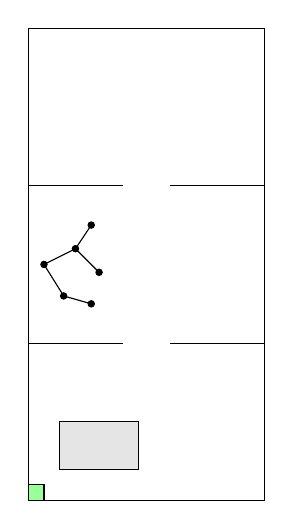
\begin{tikzpicture}
		\filldraw[fill = green!40!white, draw = black] (0, 0) rectangle (0.2, 0.2);
		\filldraw[fill = black!10!white, draw = black] (0.4, 0.4) rectangle (1.4, 1);
		\draw (0, 0) -- (3, 0) -- (3, 6) -- (0, 6) -- (0, 0);
		\draw (0, 2) -- (1.2, 2) (1.8, 2) -- (3, 2);
		\draw (0, 4) -- (1.2, 4) (1.8, 4) -- (3, 4);
		\filldraw[black] (0.2, 3) circle (0.4mm);
		\filldraw[black] (0.6, 3.2) circle (0.4mm);
		\draw (0.2,3) -- (0.6, 3.2);
		\filldraw[black] (0.45, 2.6) circle (0.4mm);
		\draw (0.2,3) -- (0.45, 2.6);
		\filldraw[black] (0.8, 3.5) circle (0.4mm);
		\draw (0.6,3.2) -- (0.8, 3.5);
		\filldraw[black] (0.9, 2.9) circle (0.4mm);
		\draw (0.6,3.2) -- (0.9, 2.9);
		\filldraw[black] (0.8, 2.5) circle (0.4mm);
		\draw (0.45, 2.6) -- (0.8, 2.5);
		\end{tikzpicture}
	\end{center}
\end{frame}

\begin{frame}
	\frametitle{RRG}
	\begin{center}
		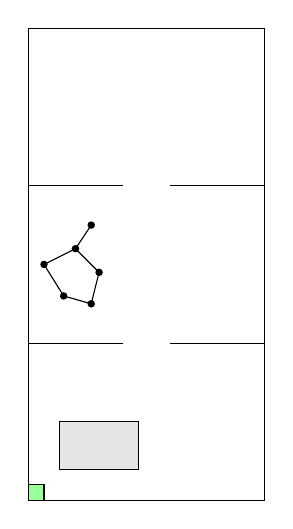
\begin{tikzpicture}
		\filldraw[fill = green!40!white, draw = black] (0, 0) rectangle (0.2, 0.2);
		\filldraw[fill = black!10!white, draw = black] (0.4, 0.4) rectangle (1.4, 1);
		\draw (0, 0) -- (3, 0) -- (3, 6) -- (0, 6) -- (0, 0);
		\draw (0, 2) -- (1.2, 2) (1.8, 2) -- (3, 2);
		\draw (0, 4) -- (1.2, 4) (1.8, 4) -- (3, 4);
		\filldraw[black] (0.2, 3) circle (0.4mm);
		\filldraw[black] (0.6, 3.2) circle (0.4mm);
		\draw (0.2,3) -- (0.6, 3.2);
		\filldraw[black] (0.45, 2.6) circle (0.4mm);
		\draw (0.2,3) -- (0.45, 2.6);
		\filldraw[black] (0.8, 3.5) circle (0.4mm);
		\draw (0.6,3.2) -- (0.8, 3.5);
		\filldraw[black] (0.9, 2.9) circle (0.4mm);
		\draw (0.6,3.2) -- (0.9, 2.9);
		\filldraw[black] (0.8, 2.5) circle (0.4mm);
		\draw (0.45, 2.6) -- (0.8, 2.5);
		\draw (0.9, 2.9) -- (0.8, 2.5);
		\end{tikzpicture}
	\end{center}
\end{frame}

\begin{frame}
	\frametitle{What about LTL?}
	\begin{itemize}
		\item Algorithms already exists for LTL specifications.\\
		\pause
		\item But they only work if the robot knows the whole environment.\\
		\pause
		\item In reality, the robot know only about things inside a sensing radius and it cannot see beyond walls or obstacles.
		\pause
		\item To know the whole environment, the robot has to explore before start planning. This is usually done by a ``frontier-based" exploration.\\
		%			\pause
	\end{itemize}
	%		\vspace{10pt}
	%		\textbf{Can we do exploration and planning together?}
\end{frame}

%\begin{frame}
%	\frametitle{Frontier Exploration}
%	\begin{itemize}
%		\item Discretize the environment into a grid. \pause
%		\item Mark each cell of the grid as \textit{free}, \textit{obstacle} or \textit{unknown}. Initially all cells are \textit{unknown}. \pause
%		\item An \textit{unknown} cell is a `frontier cell' if one of its neighbours is free. \pause
%		\item A chain of frontier cells is called a \textit{frontier}. \pause
%		\item \textit{Information Gain} of a frontier depends on its size and distance from the current position of the robot.
%	\end{itemize}
%\end{frame}


\begin{frame}
	\frametitle{LTL Motion Planning}
	\begin{center}
		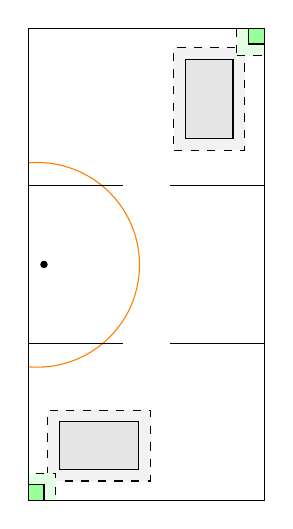
\begin{tikzpicture}
		\filldraw[dashed, fill = gray!10!white] (0.25,0.25) -- (1.55,0.25) -- (1.55,1.15) -- (0.25,1.15) -- (0.25, 0.25);
		\filldraw[dashed, fill = green!10!white] (0,0) -- (0.35,0) -- (0.35,0.35) -- (0,0.35) -- (0,0);
		\filldraw[dashed, fill = gray!10!white] (1.85,4.45) -- (2.75,4.45) -- (2.75,5.75) -- (1.85,5.75) -- (1.85, 4.45);
		\filldraw[dashed, fill = green!10!white] (2.65,5.65) -- (3,5.65) -- (3,6) -- (2.65,6) -- (2.65,5.65);
		
		\filldraw[fill = green!40!white, draw = black] (0, 0) rectangle (0.2, 0.2);
		\filldraw[fill = black!10!white, draw = black] (0.4, 0.4) rectangle (1.4, 1);
		\filldraw[fill = green!40!white, draw = black] (2.8, 5.8) rectangle (3, 6);
		\filldraw[fill = black!10!white, draw = black] (2, 4.6) rectangle (2.6, 5.6);
		
		\draw[orange] (0,1.7) arc (-95:95:1.3);
		
		\draw (0, 0) -- (3, 0) -- (3, 6) -- (0, 6) -- (0, 0);
		\draw (0, 2) -- (1.2, 2) (1.8, 2) -- (3, 2);
		\draw (0, 4) -- (1.2, 4) (1.8, 4) -- (3, 4);
		\filldraw[black] (0.2, 3) circle (0.4mm);
		\end{tikzpicture}
%		\vspace{5pt}
		\\ \emph{Specification:} $F (r_1 \wedge b) \wedge F (r_2 \wedge b)$
	\end{center}
\end{frame}

\section{Naive Algorithm}

\begin{frame}
	\frametitle{Naive Solution}
	\begin{itemize}
		\item Explore the whole environment initially using frontier based approaches. \pause
		\item Start building the RRG graph and construct an abstraction of the system on-the-fly. \pause
		\item Construct the product automaton with the property automaton. \pause
		\item Find an accepting path in the product. \pause
		\item Lift this path to the original environment.
	\end{itemize}
\end{frame}

%	\begin{frame}
%		\frametitle{Better Solution}
%		Can we do better?\\ \pause \vspace{10pt}
%		\textbf{Jan's idea:} Get help in sampling from current abstraction. \\
%		Depending on previous experiences. In other words, predict which samples would be better from previous samples. \\ \pause \vspace{10pt}
%		For e.g: The bin was close to the table in first room so try to look close to the table in the other room to find the bin.
%	\end{frame}



\begin{frame}
	\frametitle{Can we do better?}
	\begin{itemize}
		\item Too much effort is wasted in exploration. \pause
		\item Can we do exploration while trying to satisfy the path simultaneously? \pause
		\item Identify places to go to, so that there is some progress in satisfying the property.
	\end{itemize}
\end{frame}


\section{Better Solution}

\begin{frame}
	\frametitle{Our solution}
	\begin{itemize}
		\item Sample a batch in the known area (initially, sensing radius) using biasing (initially, no biasing).
		\only<2-3>{
			\item Learn from the newly added edges and improve the bias.
		}
		\only<4>{
			\item \textcolor{red}{Learn from the newly added edges and improve the bias.}
		}
		\onslide<3->{
			\item Find the best move and go there.
			\vspace{10pt}
		}
		\onslide<2>{
			\begin{figure}
				\centering
				\scalebox{.5}{
					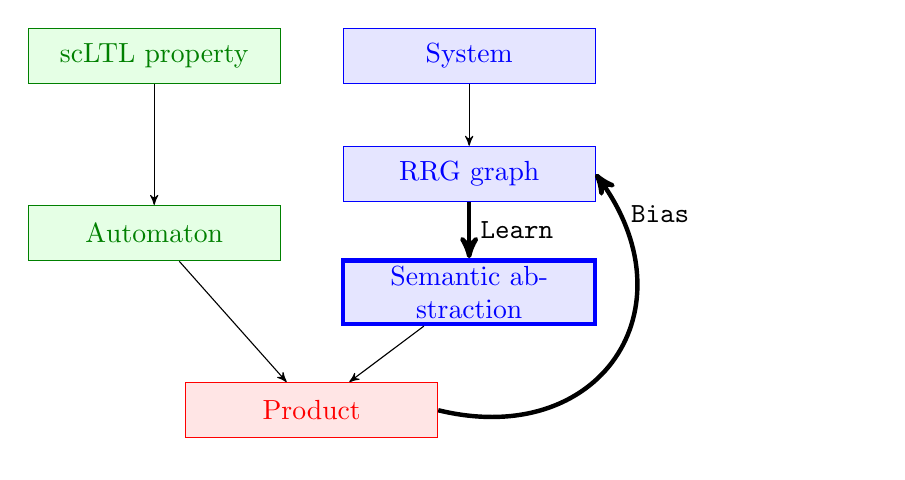
\begin{tikzpicture}[->,>=stealth', minimum width = 32mm,text width = 30mm, state/.style={
						rectangle,
						%   rounded corners,
						draw=black, very thick,
						minimum height=2em,
						inner sep=2pt,
						text centered,
					},]
					\node[state=initial, color = blue, anchor=center, fill = blue!10!white,thin] (A) {System};
					\node[state, color = blue, below of = A, fill = blue!10!white, node distance =1.5cm,thin] (B) {RRG graph};
					\node[state, color = blue, below of = B, fill = blue!10!white, node distance =1.5cm,ultra thick] (C) {Semantic abstraction};
					\node[state, color = red, below of = C, fill = red!10!white, xshift = -2cm, node distance =1.5cm,thin] (D) {Product};
					\node[state, color = green!50!black, left of = A, fill = green!10!white, node distance =4cm,thin] (E) {scLTL property};
					\node[state, color = green!50!black, below of = E, fill = green!10!white, node distance =2.25cm,thin] (F) {Automaton};
					
					\path (A) edge[] (B)
					(B) edge[ultra thick] node[right,pos=0.5]{\texttt{Learn}} (C)
					(C) edge (D)
					(E) edge (F)
					(F) edge (D)
					(D.east) edge[bend right=70,looseness=1.5, ultra thick] node[right,pos=0.9]{\texttt{Bias}} (B.east)
					%guidance $\rightarrow$ better paths and learning w.r.t. property
					;
					\end{tikzpicture}
				}
				%					\caption{Scheme of our model-checking-inspired approach with novel elements drawn thickly. }
				\label{fig:guide}
			\end{figure}
		}
	\end{itemize}
\end{frame}


\begin{frame}
	\frametitle{Learn and Bias}
	\begin{itemize}
		\item Learn from past experiences i.e. look for transitions that are similar to transitions that we have seen till now. \pause
		\item For each transition sampled in the current batch, add similar `maybe' transitions in the abstraction as well. \pause
		\item Use these `maybe' transitions to bias the search.
	\end{itemize}
\end{frame}

\begin{frame}
	\frametitle{Learn and Bias}
	\begin{itemize}
		\item What does similar mean here?\\
		$(r_1, t) \rightarrow (r_1, b) \implies (r_2, t) \rightarrow (r_2,b)$. \\
		\begin{itemize}
			\item Compute domain of changes: Set of APs changing in a transition.\\
			$DOC = \{t,b\}$, $(s_1 \oplus s_2)$
			\item Add transitions $s_1' \rightarrow s_2'$ where $s_1'$ and $s_2'$ are states which agree with $s_1$ and $s_2$ on $DOC$ respectively.
		\end{itemize}
	\end{itemize}
\end{frame}

\begin{frame}
	\frametitle{Example}
	\begin{center}
		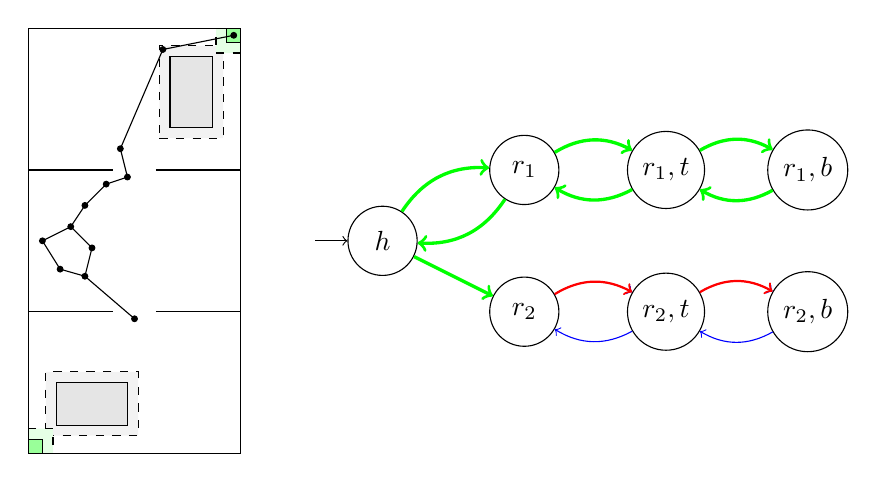
\begin{tikzpicture}[scale = 0.9]
		\filldraw[dashed, fill = gray!10!white] (0.25,0.25) -- (1.55,0.25) -- (1.55,1.15) -- (0.25,1.15) -- (0.25, 0.25);
		\filldraw[dashed, fill = green!10!white] (0,0) -- (0.35,0) -- (0.35,0.35) -- (0,0.35) -- (0,0);
		\filldraw[dashed, fill = gray!10!white] (1.85,4.45) -- (2.75,4.45) -- (2.75,5.75) -- (1.85,5.75) -- (1.85, 4.45);
		\filldraw[dashed, fill = green!10!white] (2.65,5.65) -- (3,5.65) -- (3,6) -- (2.65,6) -- (2.65,5.65);
		
		\filldraw[fill = green!40!white, draw = black] (0, 0) rectangle (0.2, 0.2);
		\filldraw[fill = black!10!white, draw = black] (0.4, 0.4) rectangle (1.4, 1);
		\filldraw[fill = green!40!white, draw = black] (2.8, 5.8) rectangle (3, 6);
		\filldraw[fill = black!10!white, draw = black] (2, 4.6) rectangle (2.6, 5.6);
		
		\draw (0, 0) -- (3, 0) -- (3, 6) -- (0, 6) -- (0, 0);
		\draw (0, 2) -- (1.2, 2) (1.8, 2) -- (3, 2);
		\draw (0, 4) -- (1.2, 4) (1.8, 4) -- (3, 4);
		\filldraw[black] (0.2, 3) circle (0.4mm);
		
		%			\onslide<2->{
		%				\node[state,initial,initial text=,scale=0.8] (q1) at (5,5) {$0$};
		%				\node[state,scale=0.8] (q2) at (8,5) {$1$};
		%				
		%				\draw (q1) edge[loop above] node{$r_1 \wedge r_2 \wedge b\ \ast$} (q1);
		%				\draw (q1) edge[loop below] node{$(r_1 \wedge \neg b) \vee \neg r_1$} (q1);
		%				\draw (q1) edge[bend left, above, ->] node{$r_1 \wedge \neg r_2 \wedge b$} (q2);
		%				\draw (q2) edge[loop above] node{$(r_2 \wedge b) \vee \neg r_1$} (q2);
		%				\draw (q2) edge[bend left, below, ->] node{$r_2 \wedge b\ \ast$} (q1);
		%			}
		
		\onslide<2->{
			\filldraw[black] (0.6, 3.2) circle (0.4mm);
			\draw (0.2,3) -- (0.6, 3.2);
			\filldraw[black] (0.45, 2.6) circle (0.4mm);
			\draw (0.2,3) -- (0.45, 2.6);
			\filldraw[black] (0.8, 3.5) circle (0.4mm);
			\draw (0.6,3.2) -- (0.8, 3.5);
			\filldraw[black] (0.9, 2.9) circle (0.4mm);
			\draw (0.6,3.2) -- (0.9, 2.9);
			\filldraw[black] (0.8, 2.5) circle (0.4mm);
			\draw (0.45, 2.6) -- (0.8, 2.5);
			\draw (0.9, 2.9) -- (0.8, 2.5);
			\filldraw[black] (1.1, 3.8) circle (0.4mm);
			\draw (0.8, 3.5) -- (1.1, 3.8);
			\filldraw[black] (1.4, 3.9) circle (0.4mm);
			\draw (1.1, 3.8) -- (1.4, 3.9);
			
			\node[state,initial,initial text=] (h) at (5,3) {$h$};
			%				\draw (h) edge[loop above, color = green, very thick] node{} (h);
		}
		
		\onslide<3->{
			\filldraw[black] (1.3, 4.3) circle (0.4mm);
			\draw (1.4, 3.9) -- (1.3, 4.3);
			
			\node[state] (r1) at (7,4) {$r_1$};
			\draw (h) edge[color = green, bend left, ->, very thick] node{} (r1);
		}
		\onslide<4->{
			\filldraw[black] (1.9, 5.7) circle (0.4mm);
			\draw (1.3, 4.3) -- (1.9, 5.7);
			
			\node[state] (r1t) at (9, 4) {$r_1, t$};
			\draw (r1) edge[color = green, bend left, ->, very thick] node{} (r1t);
			
		}
		\onslide<6->{
			\node[state] (r2) at (7,2) {$r_2$};
			\node[state] (r2t) at (9, 2) {$r_2, t$};
			\draw (r2) edge[color = blue, bend left, ->] node{} (r2t);
			
		}
		\onslide<7->{
			
			\filldraw[black] (2.9, 5.9) circle (0.4mm);
			\draw (1.9, 5.7) -- (2.9, 5.9);
			\filldraw[black] (1.5, 1.9) circle (0.4mm);
			\draw (0.8, 2.5) -- (1.5, 1.9);
			
			\node[state] (r1b) at (11, 4) {$r_1, b$};
			\node[state] (r2b) at (11, 2) {$r_2, b$};
			\draw (r1) edge[color = green, bend left, ->, very thick] node{} (h);
			\draw (r1t) edge[color = green, bend left, ->, very thick] node{} (r1);
			\draw (r1t) edge[color = green, bend left, ->, very thick] node{} (r1b);
			\draw (r1b) edge[color = green, bend left, ->, very thick] node{} (r1t);
			\draw (h) edge[color = green, ->, very thick] node{} (r2);
			
			%				\draw (r2) edge[color = blue, bend left, ->] node{} (h);
			\draw (r2t) edge[color = blue, bend left, ->] node{} (r2);
			\draw (r2t) edge[color = blue, bend left, ->] node{} (r2b);
			\draw (r2b) edge[color = blue, bend left, ->] node{} (r2t);
		}
		\onslide<8->{
			\draw (r2) edge[color = red, bend left, ->, thick] node{} (r2t);
			\draw (r2t) edge[color = red, bend left, ->, thick] node{} (r2b);
			
			
		}
		
		
		\end{tikzpicture}
		\onslide<5-6>{
			$DOC = \{t\}$
		}
	\end{center}
\end{frame}

\begin{frame}
	\frametitle{Our solution}
	\begin{itemize}
		\item Sample a batch in the known area (initially, sensing radius) using biasing (initially, no biasing).
		\item Learn from the newly added edges and improve the bias. \textcolor{green}{\cmark}
		\only<1>{
			\item Find the best move and go there.
		}
		\only<2>{
			\item \textcolor{red}{Find the best move and go there.}
		}
	\end{itemize}
\end{frame}

\begin{frame}
	\frametitle{Where to move?}
	Possible options:
	\begin{itemize}
		\item One of the frontiers (as in frontier exploration).
		\item Points sampled in the current batch which were according to the bias. Define IG for these based on how far they are from the accepting state in the product automaton.
	\end{itemize}
\end{frame}

\begin{frame}
	\frametitle{Our solution}
	\begin{itemize}
		\item Sample a batch in the known area (initially, sensing radius) using biasing (initially, no biasing).
		\item Learn from the newly added edges and improve the bias. \textcolor{green}{\cmark}
		\item Find the best move and go there. \textcolor{green}{\cmark}
	\end{itemize}
\end{frame}

\section{Experiments}

\begin{frame}
	\frametitle{A run of ``First Explore Then Plan"}
	\only<1>{
		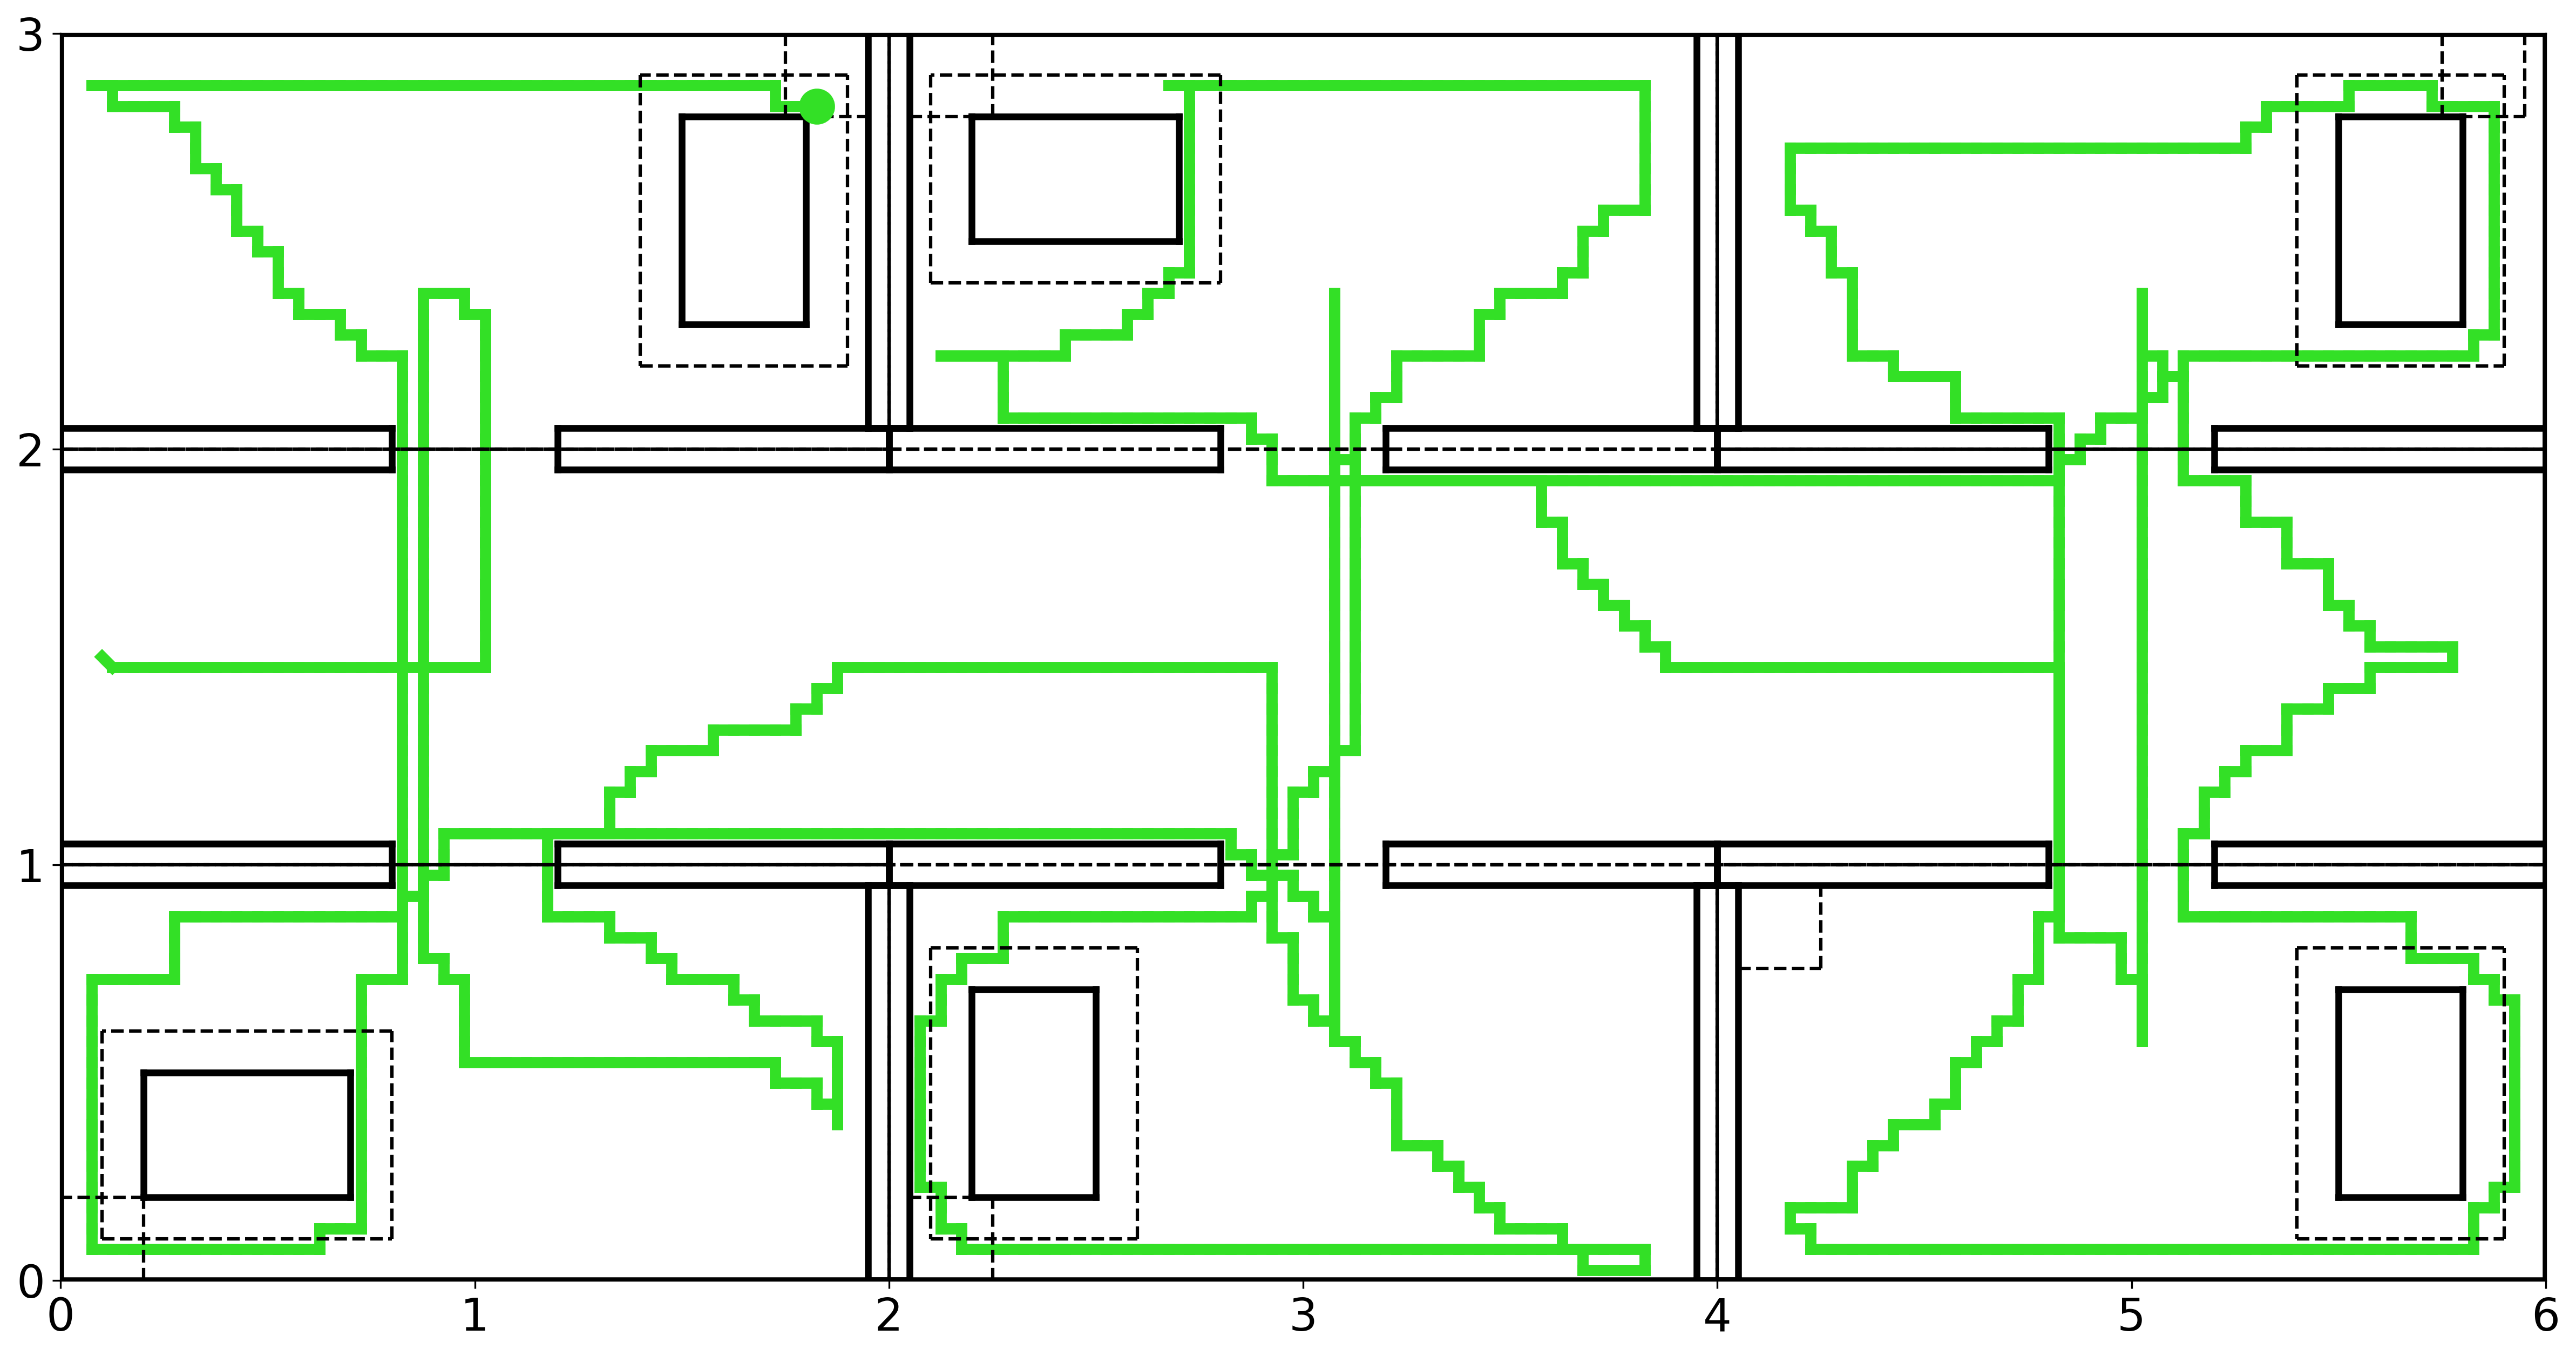
\includegraphics[width=\textwidth]{Fig/sep_bin.png}
	}
	\only<2>{
		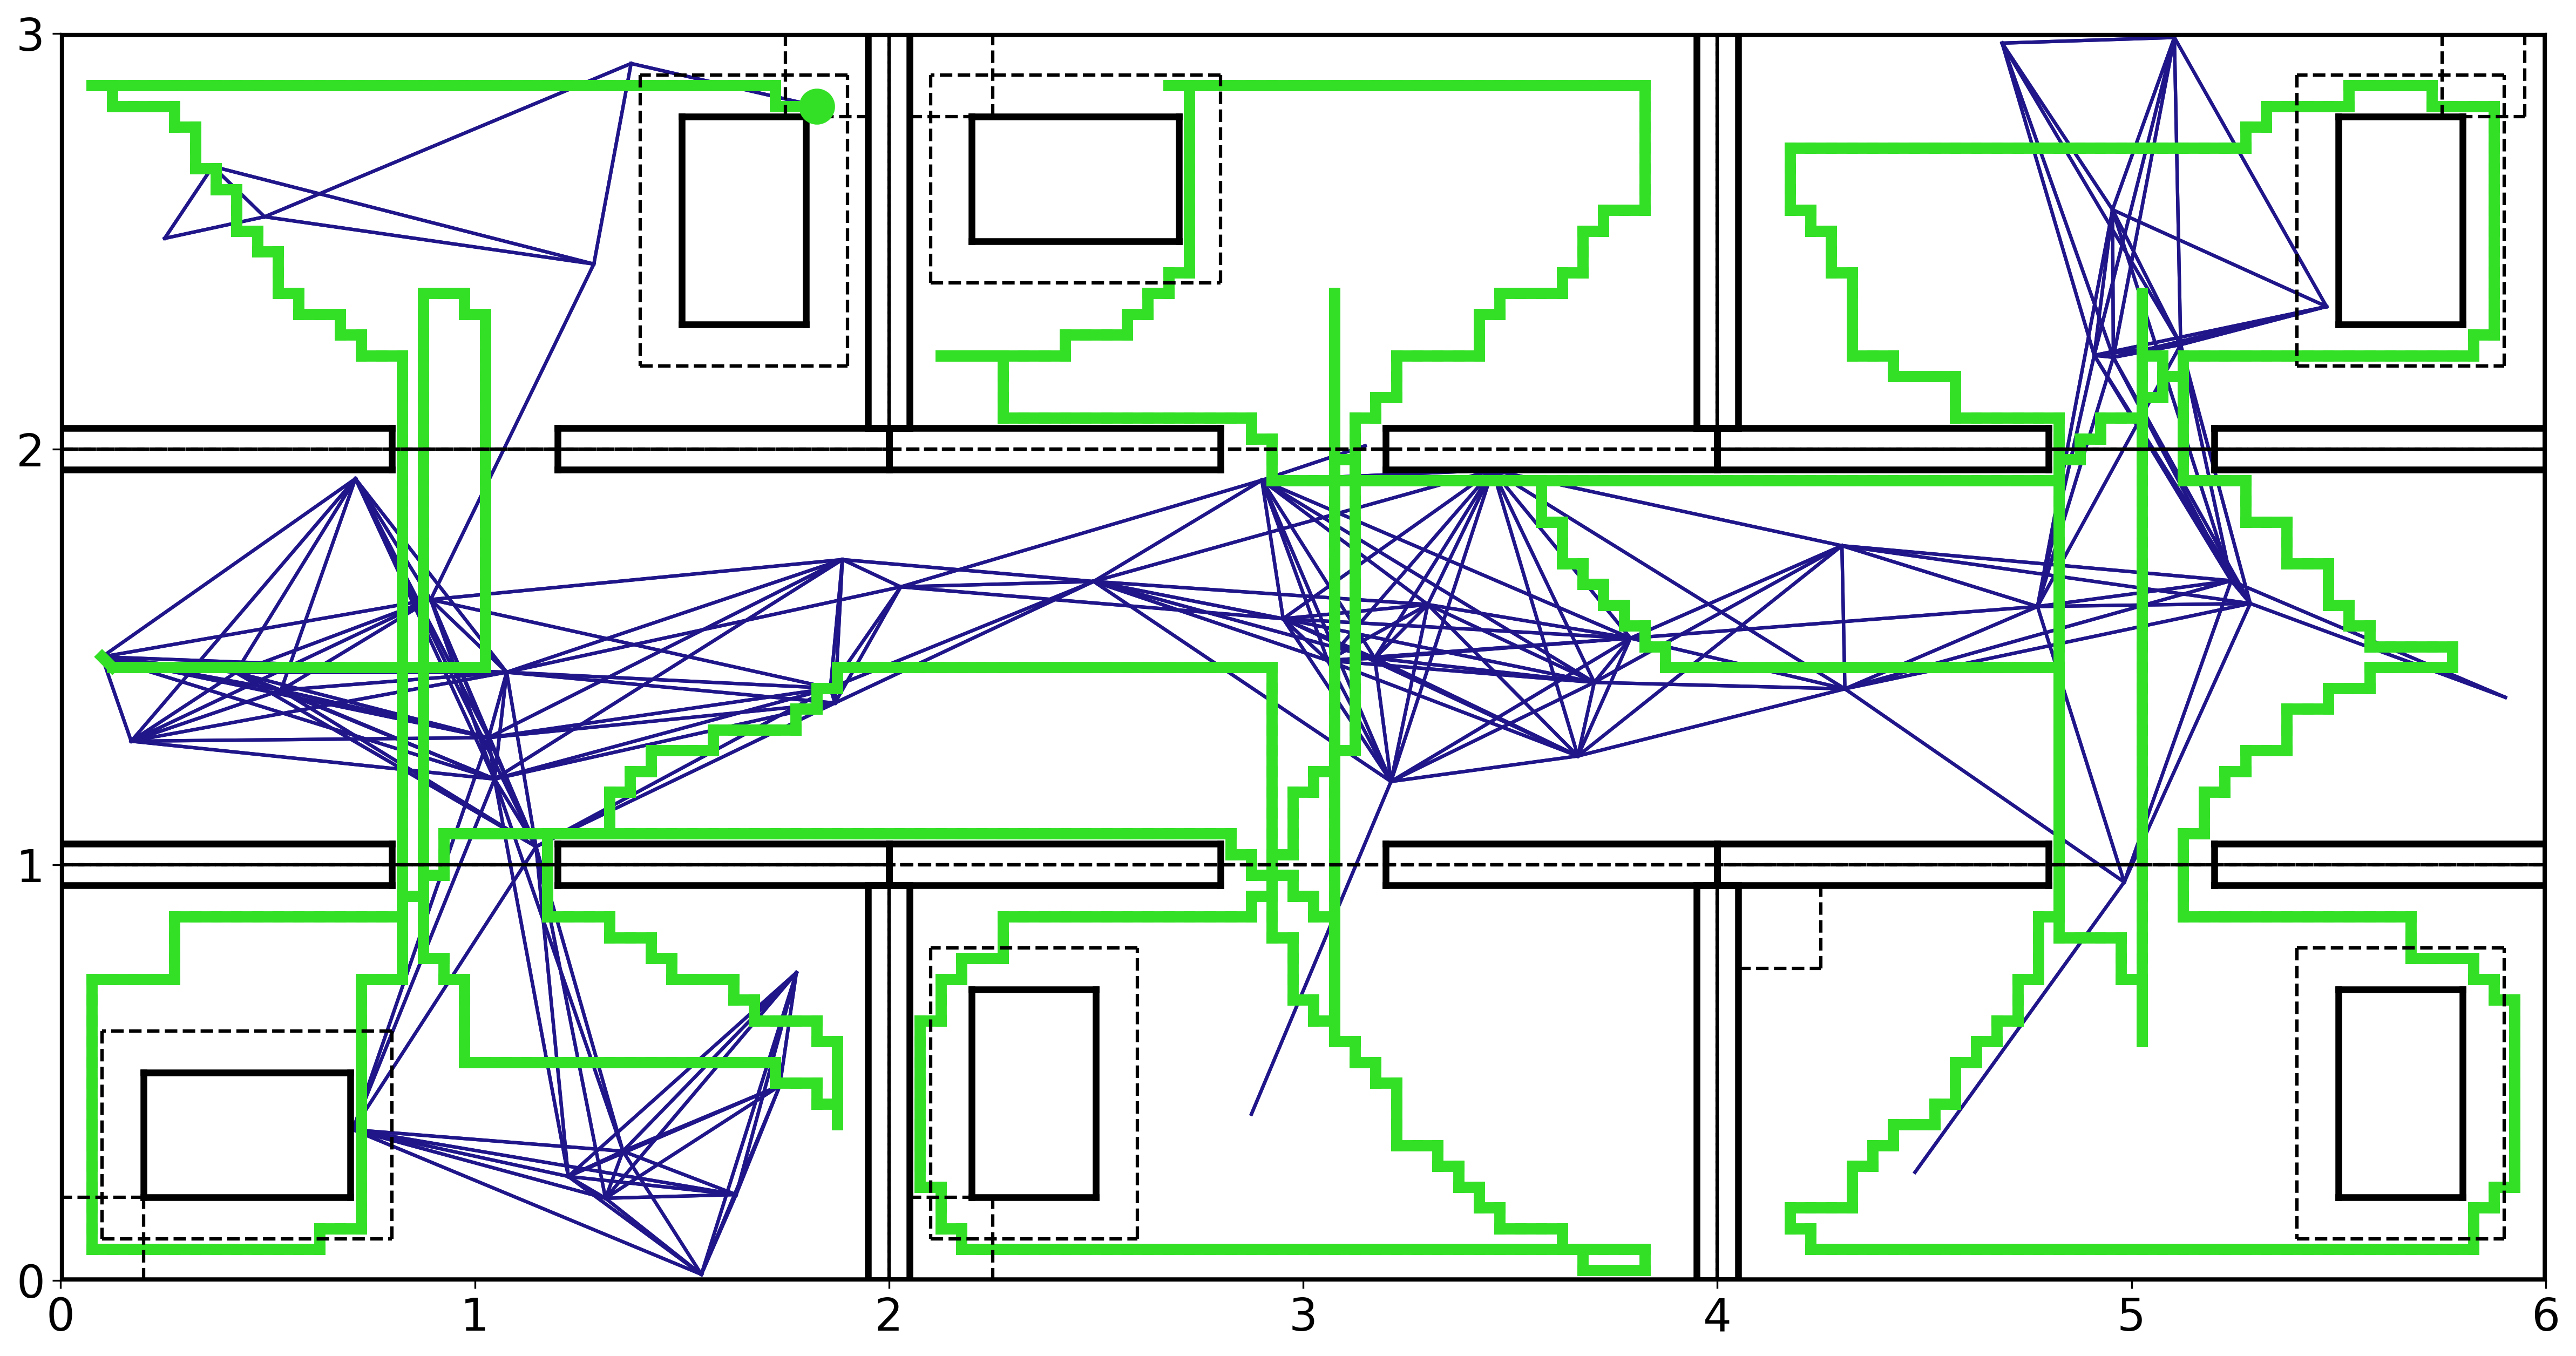
\includegraphics[width=\textwidth]{Fig/sep_room.png}
	}
	\only<3>{
		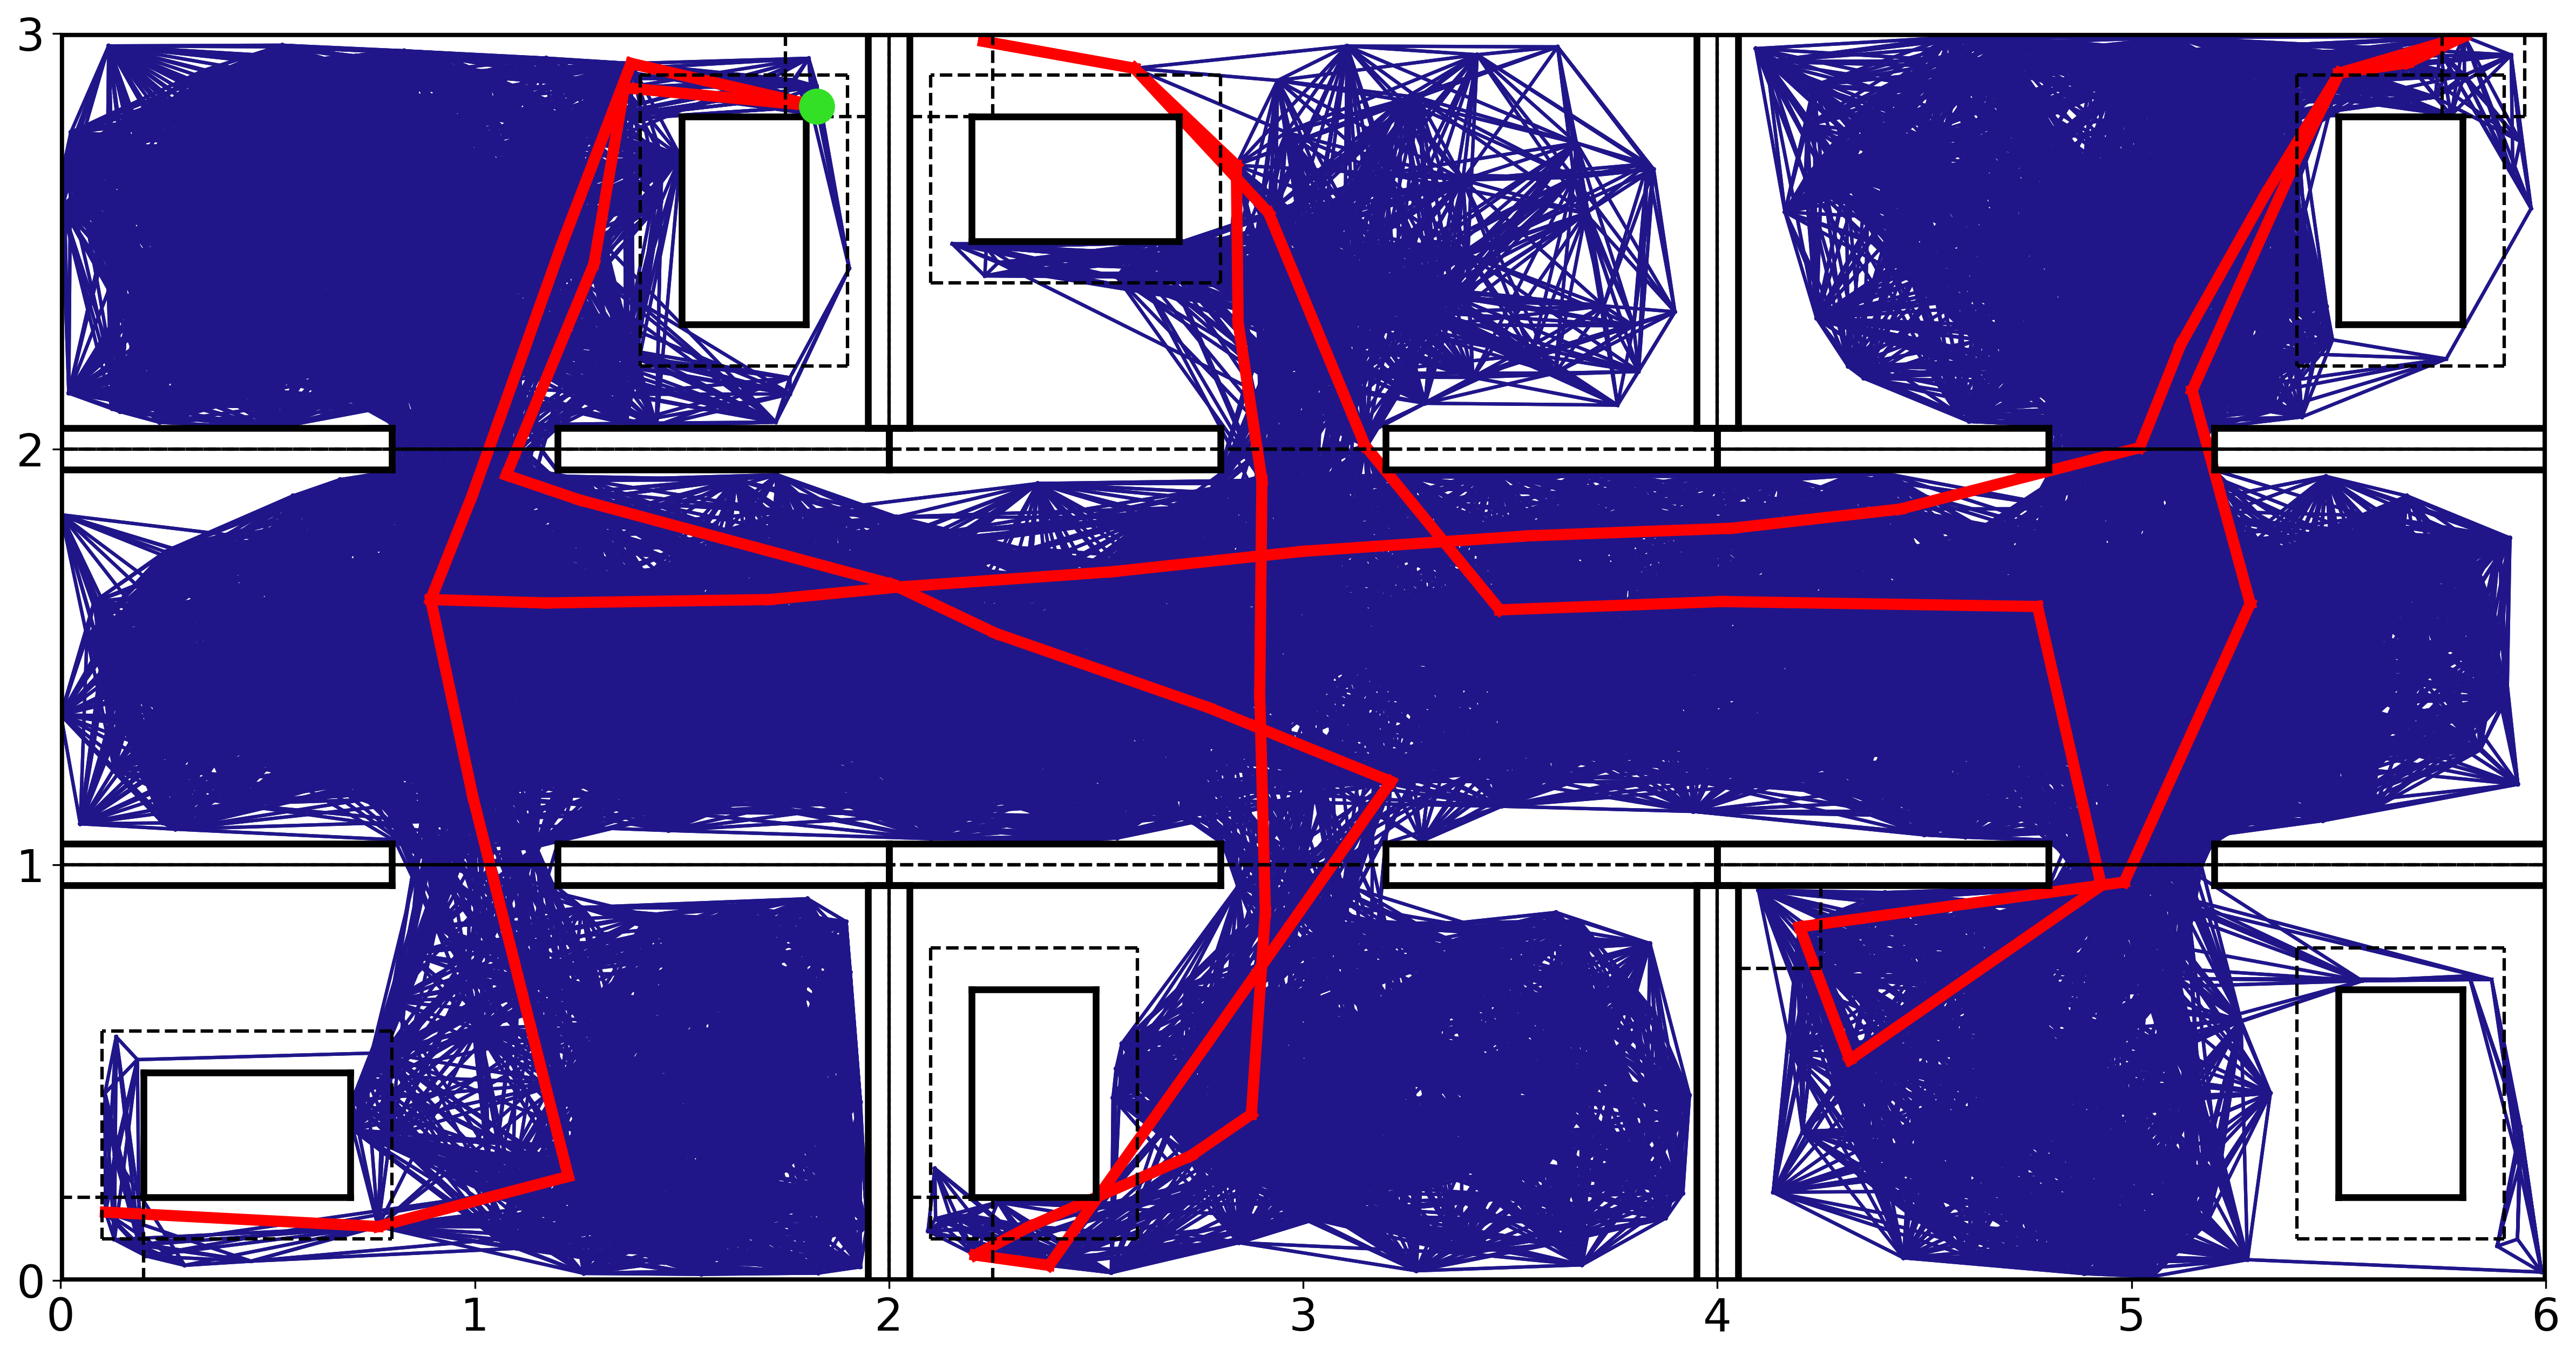
\includegraphics[width=\textwidth]{Fig/sep_final.png}
	}
\end{frame}

\begin{frame}
	\frametitle{A run of ``Simultaneously with biasing"}
	\only<1>{
		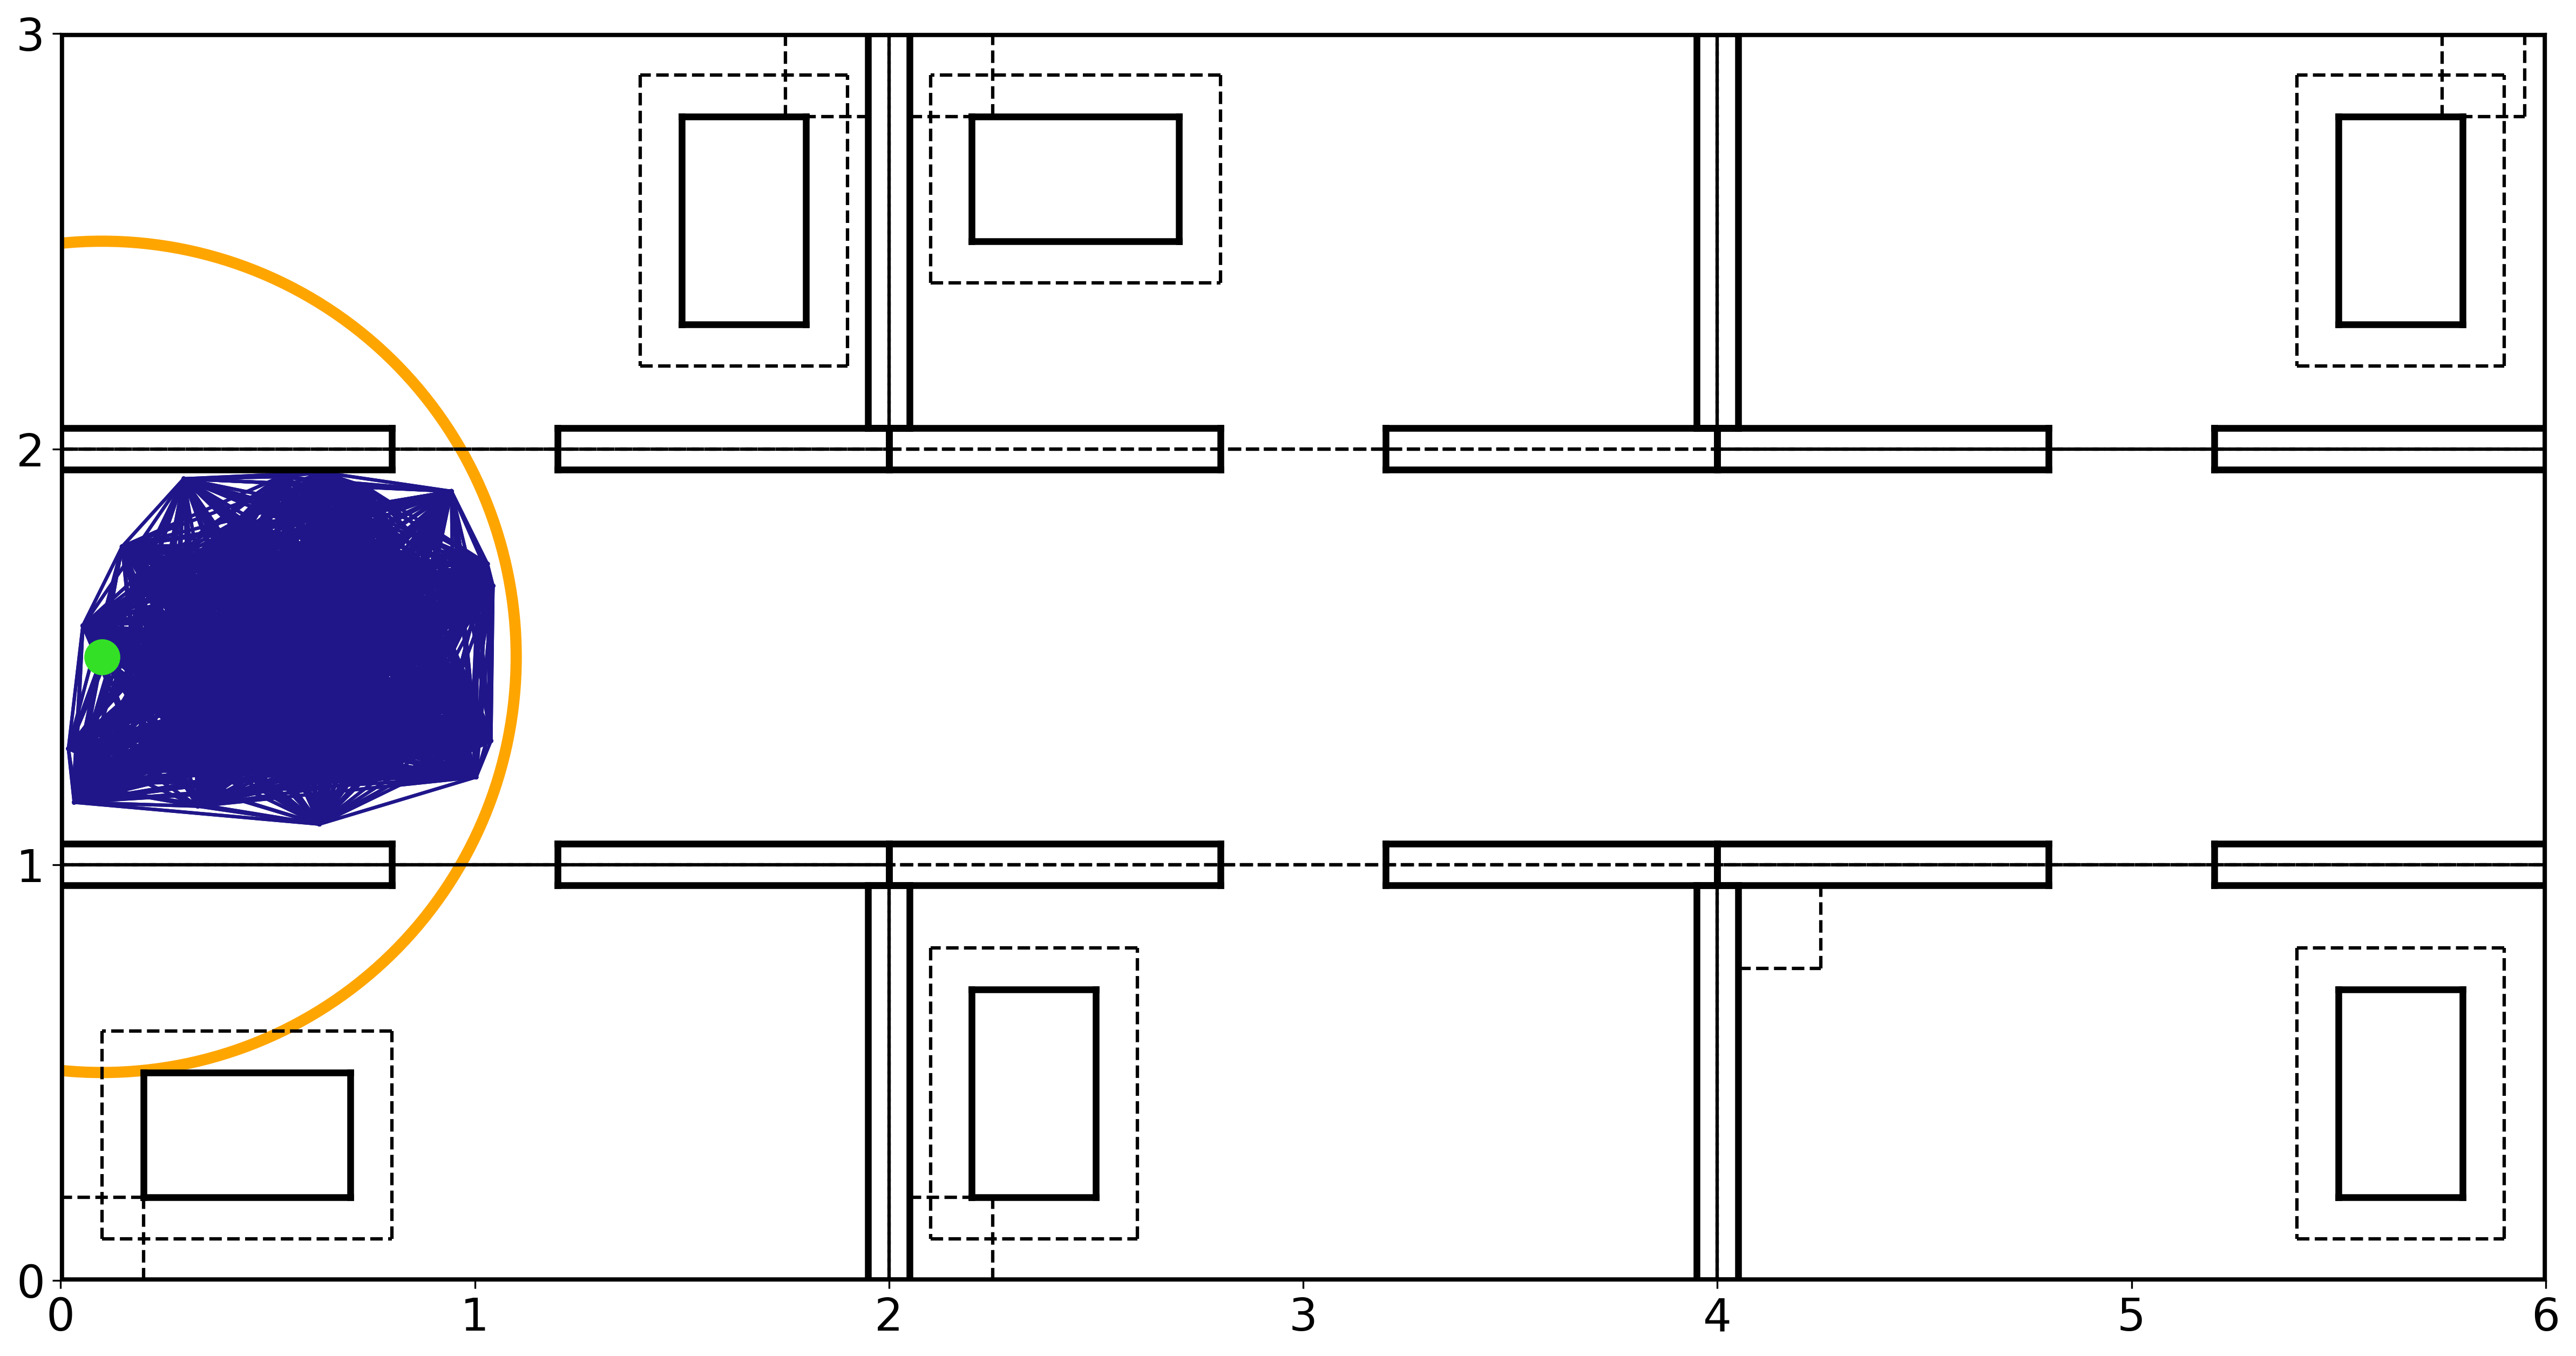
\includegraphics[width=\textwidth]{Fig/tog_firstMove.png}
	}
	\only<2>{
		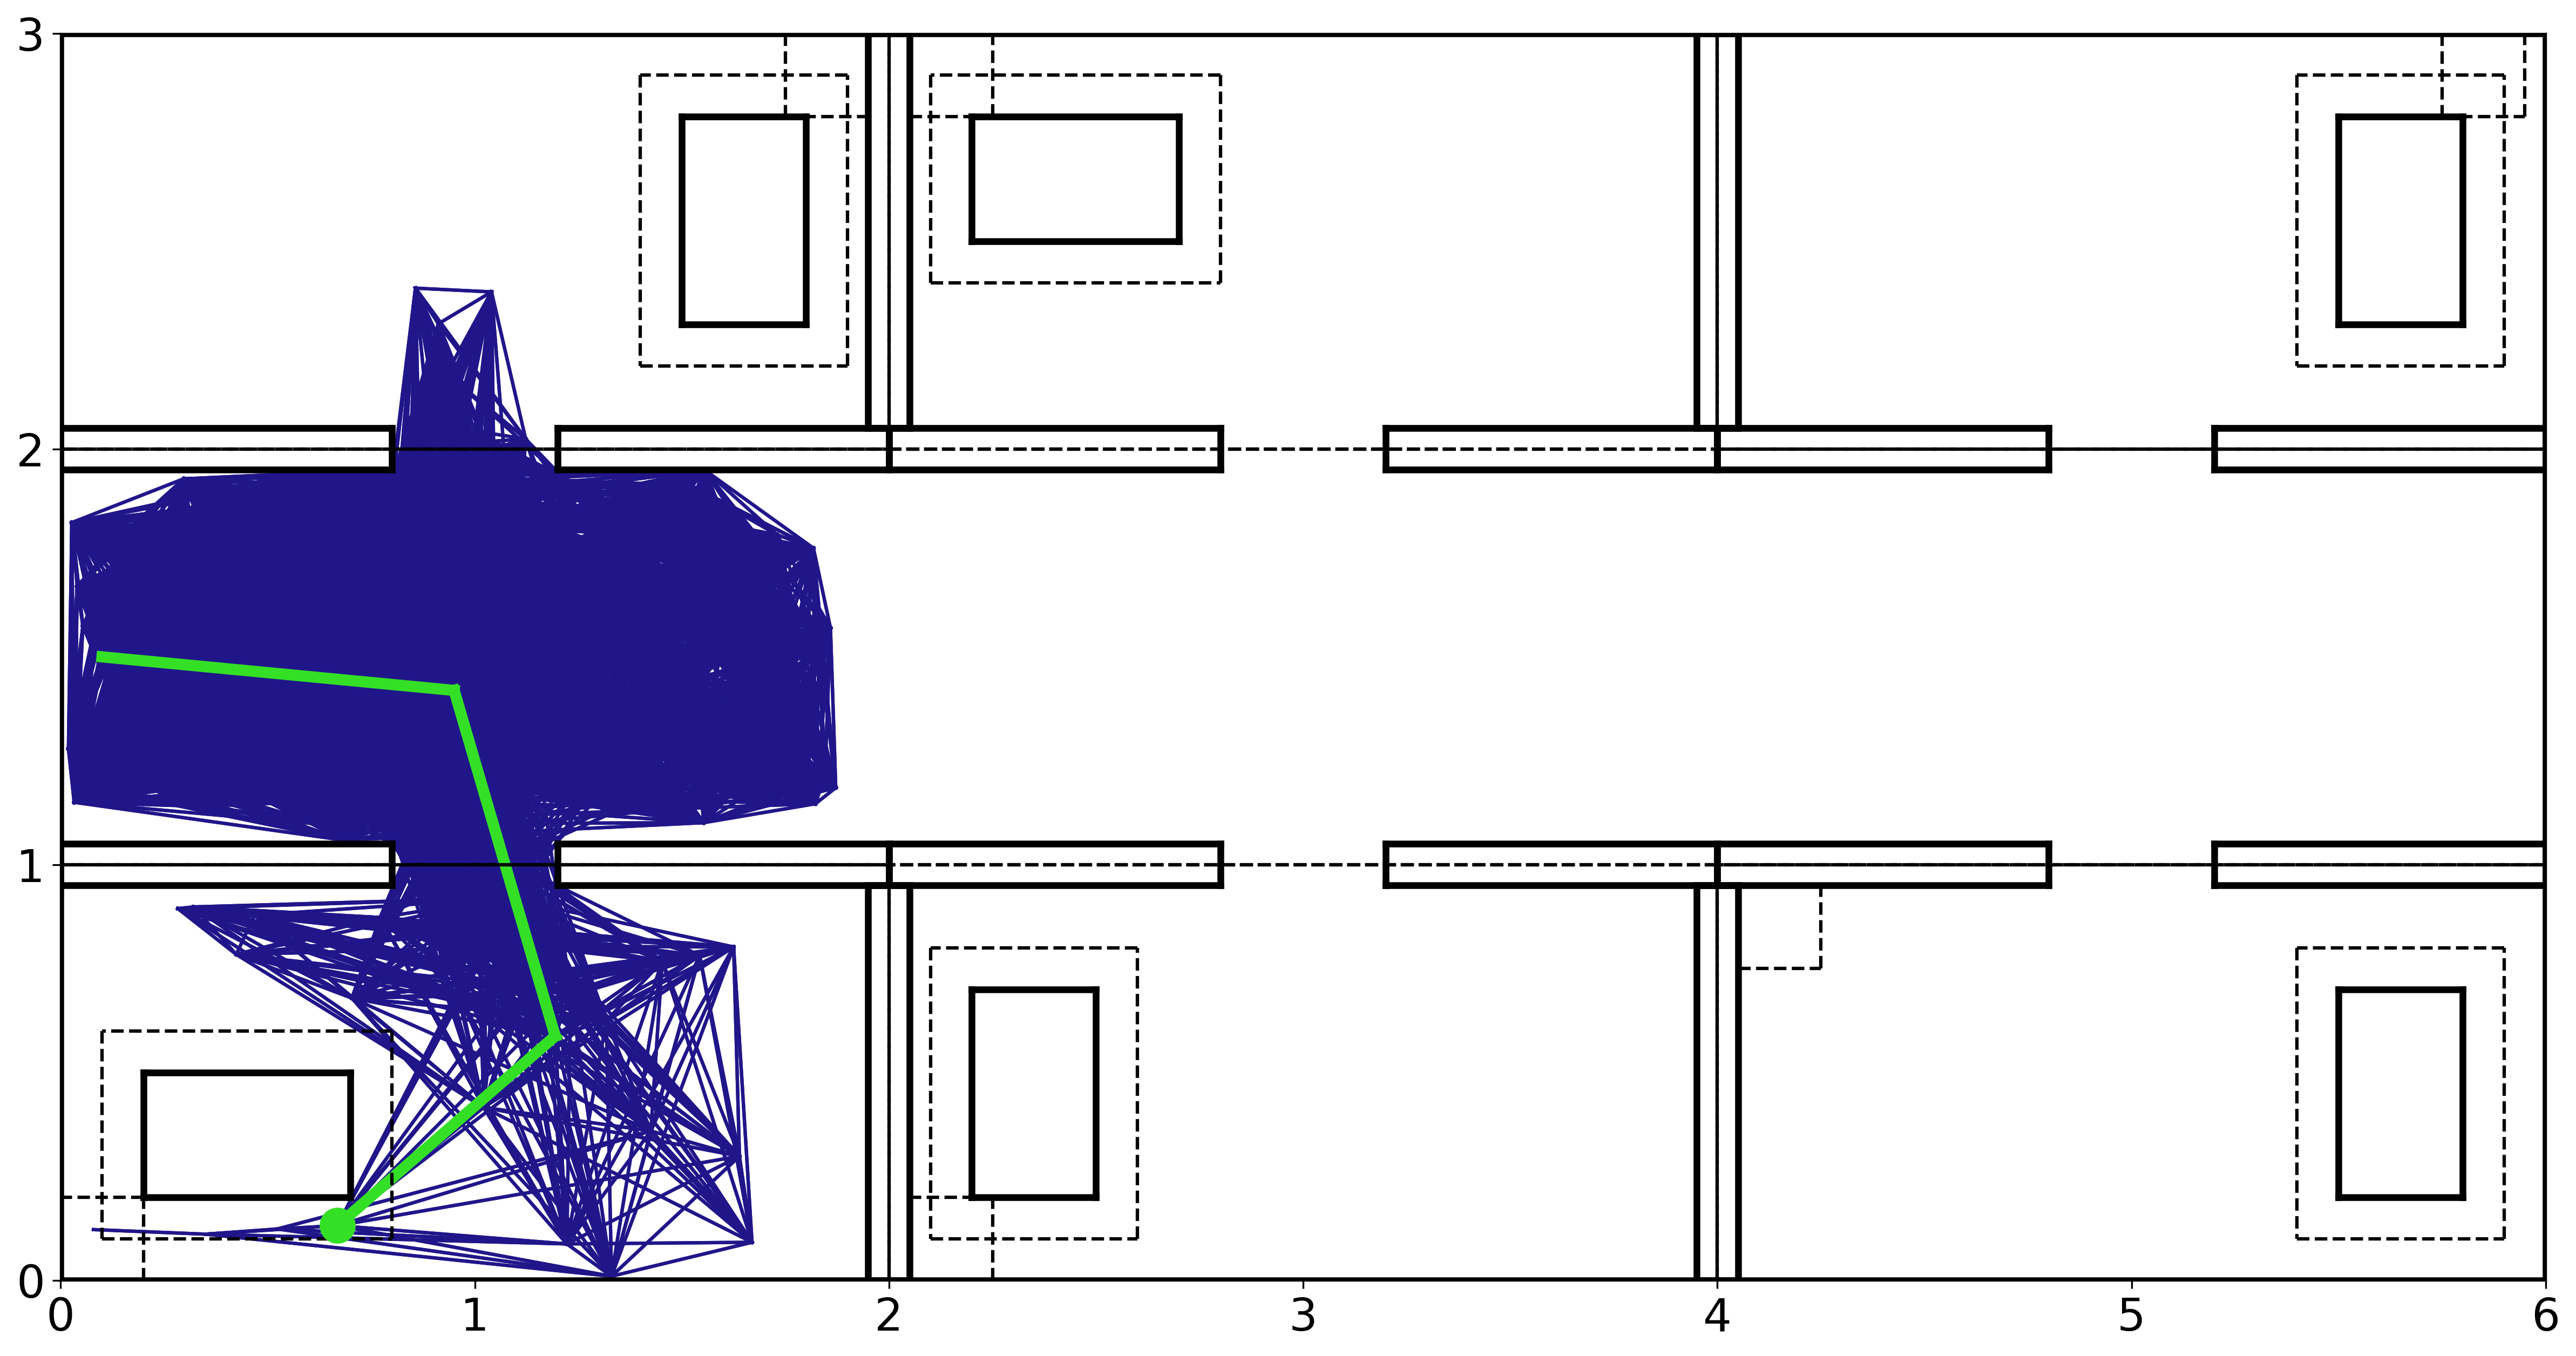
\includegraphics[width=\textwidth]{Fig/tog_bin.png}
	}
	\only<3>{
		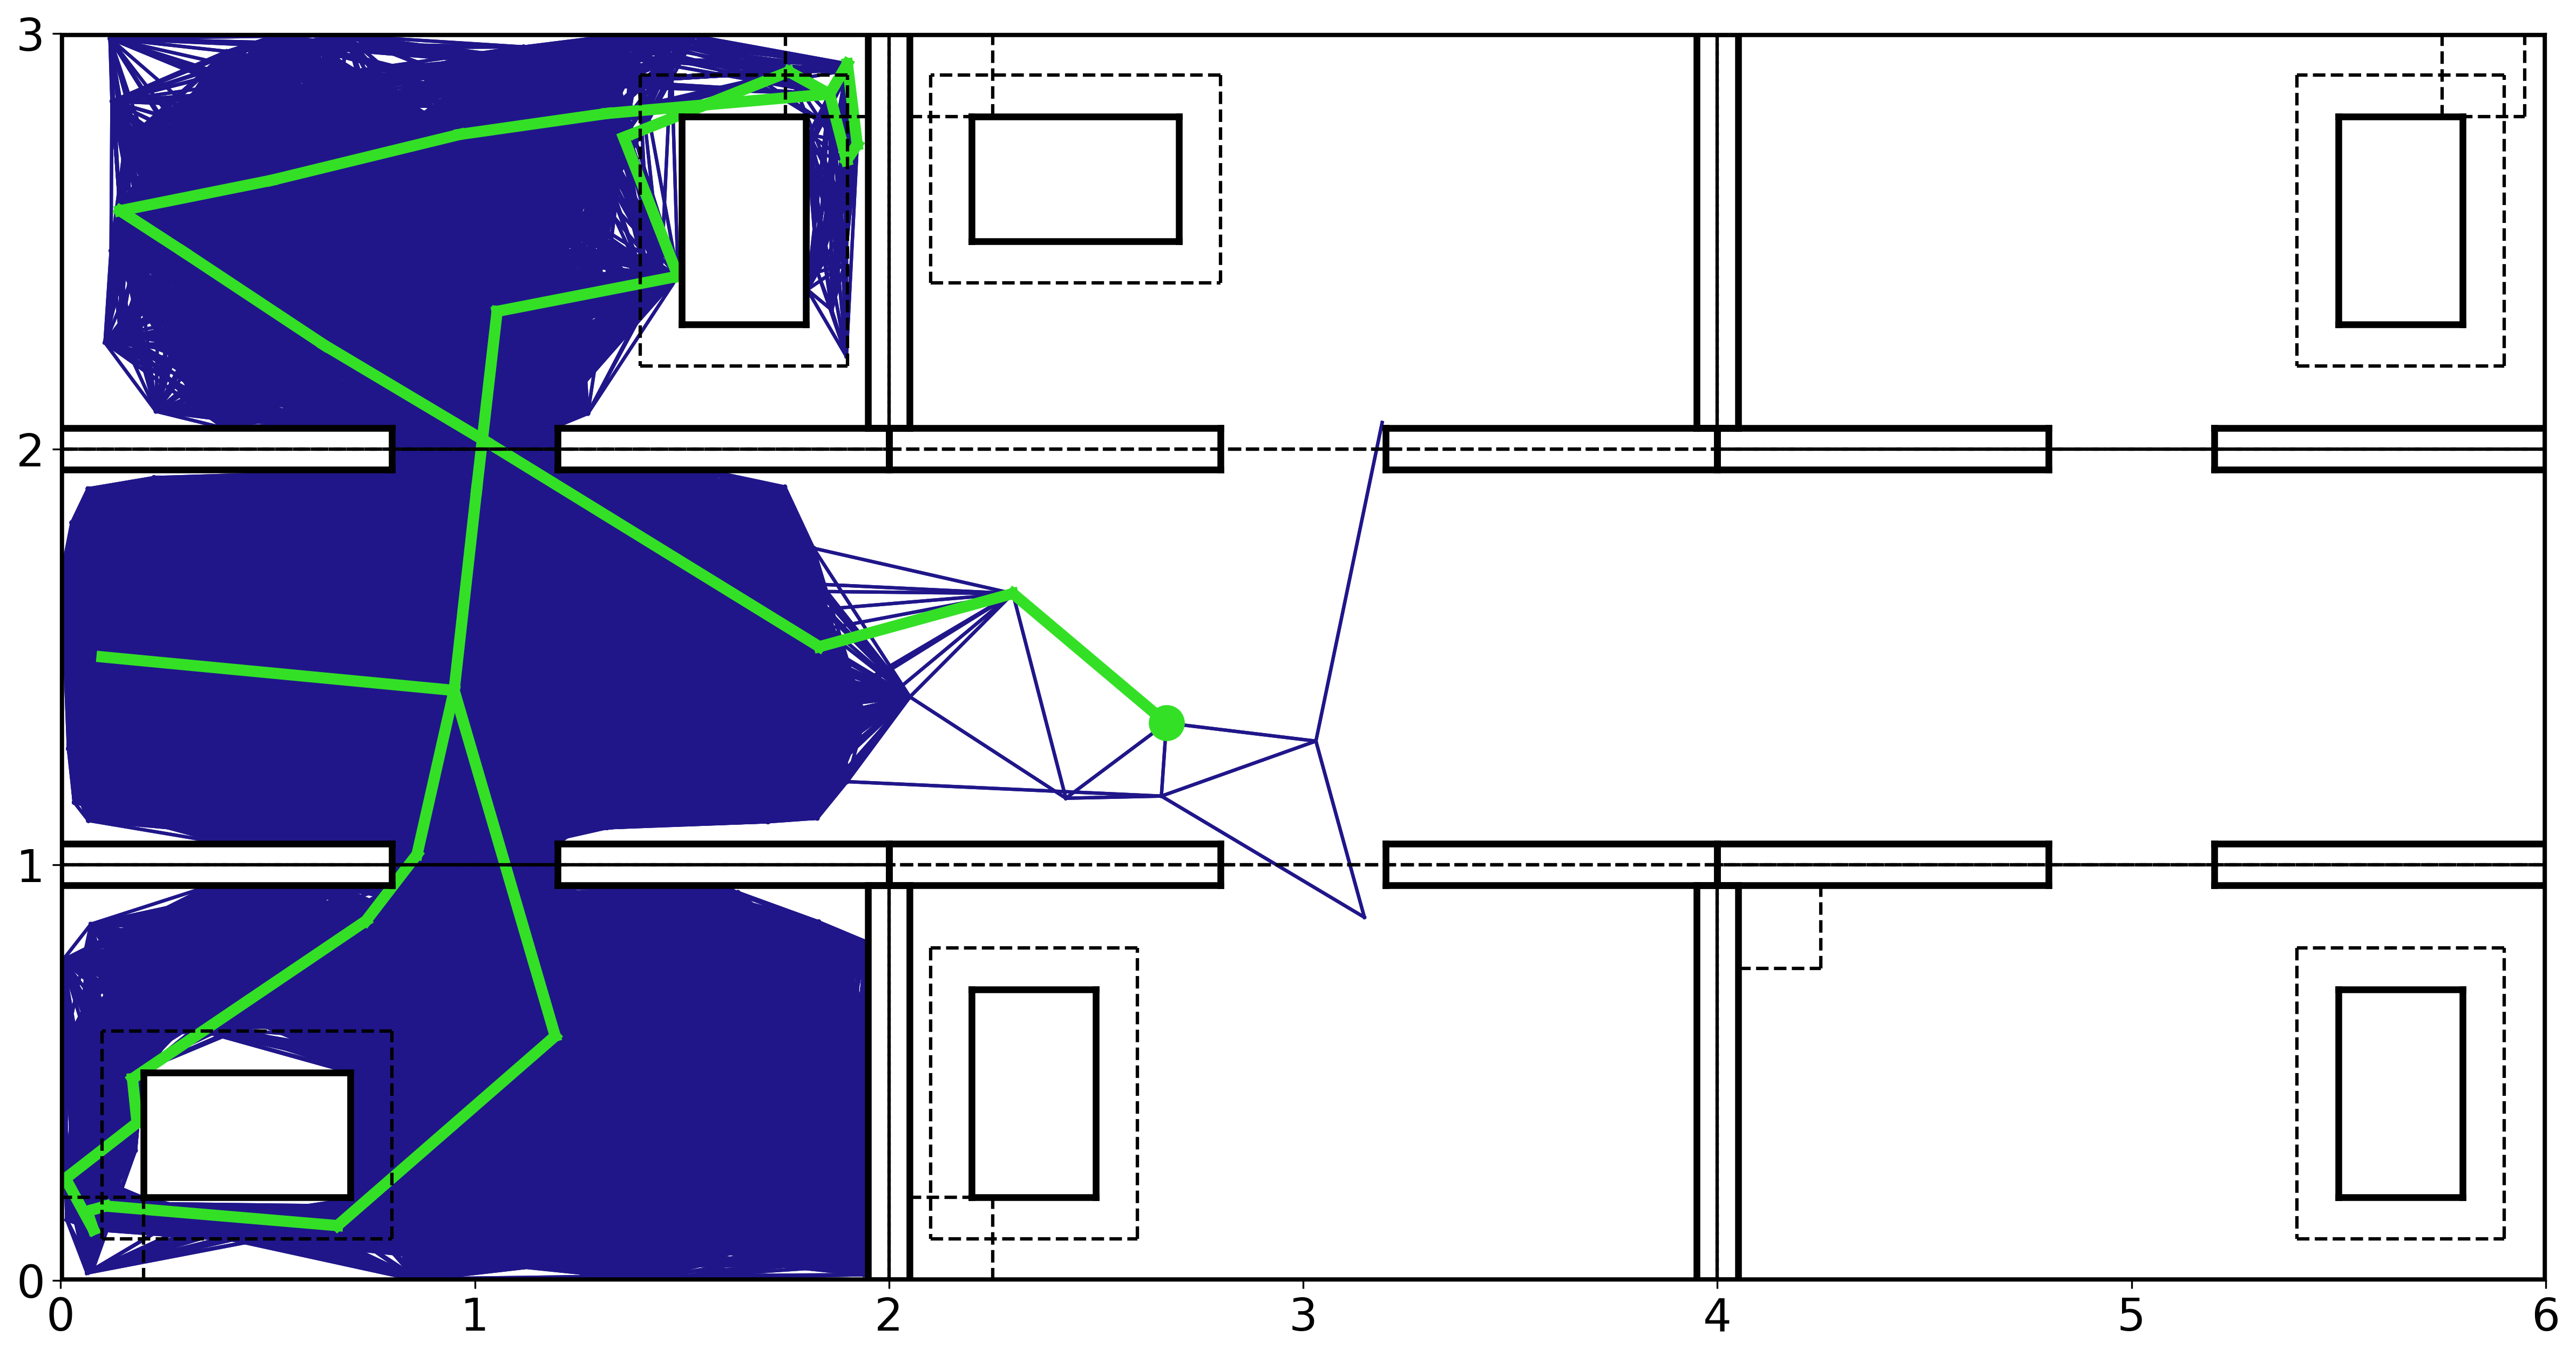
\includegraphics[width=\textwidth]{Fig/tog_room.png}
	}
	\only<4>{
		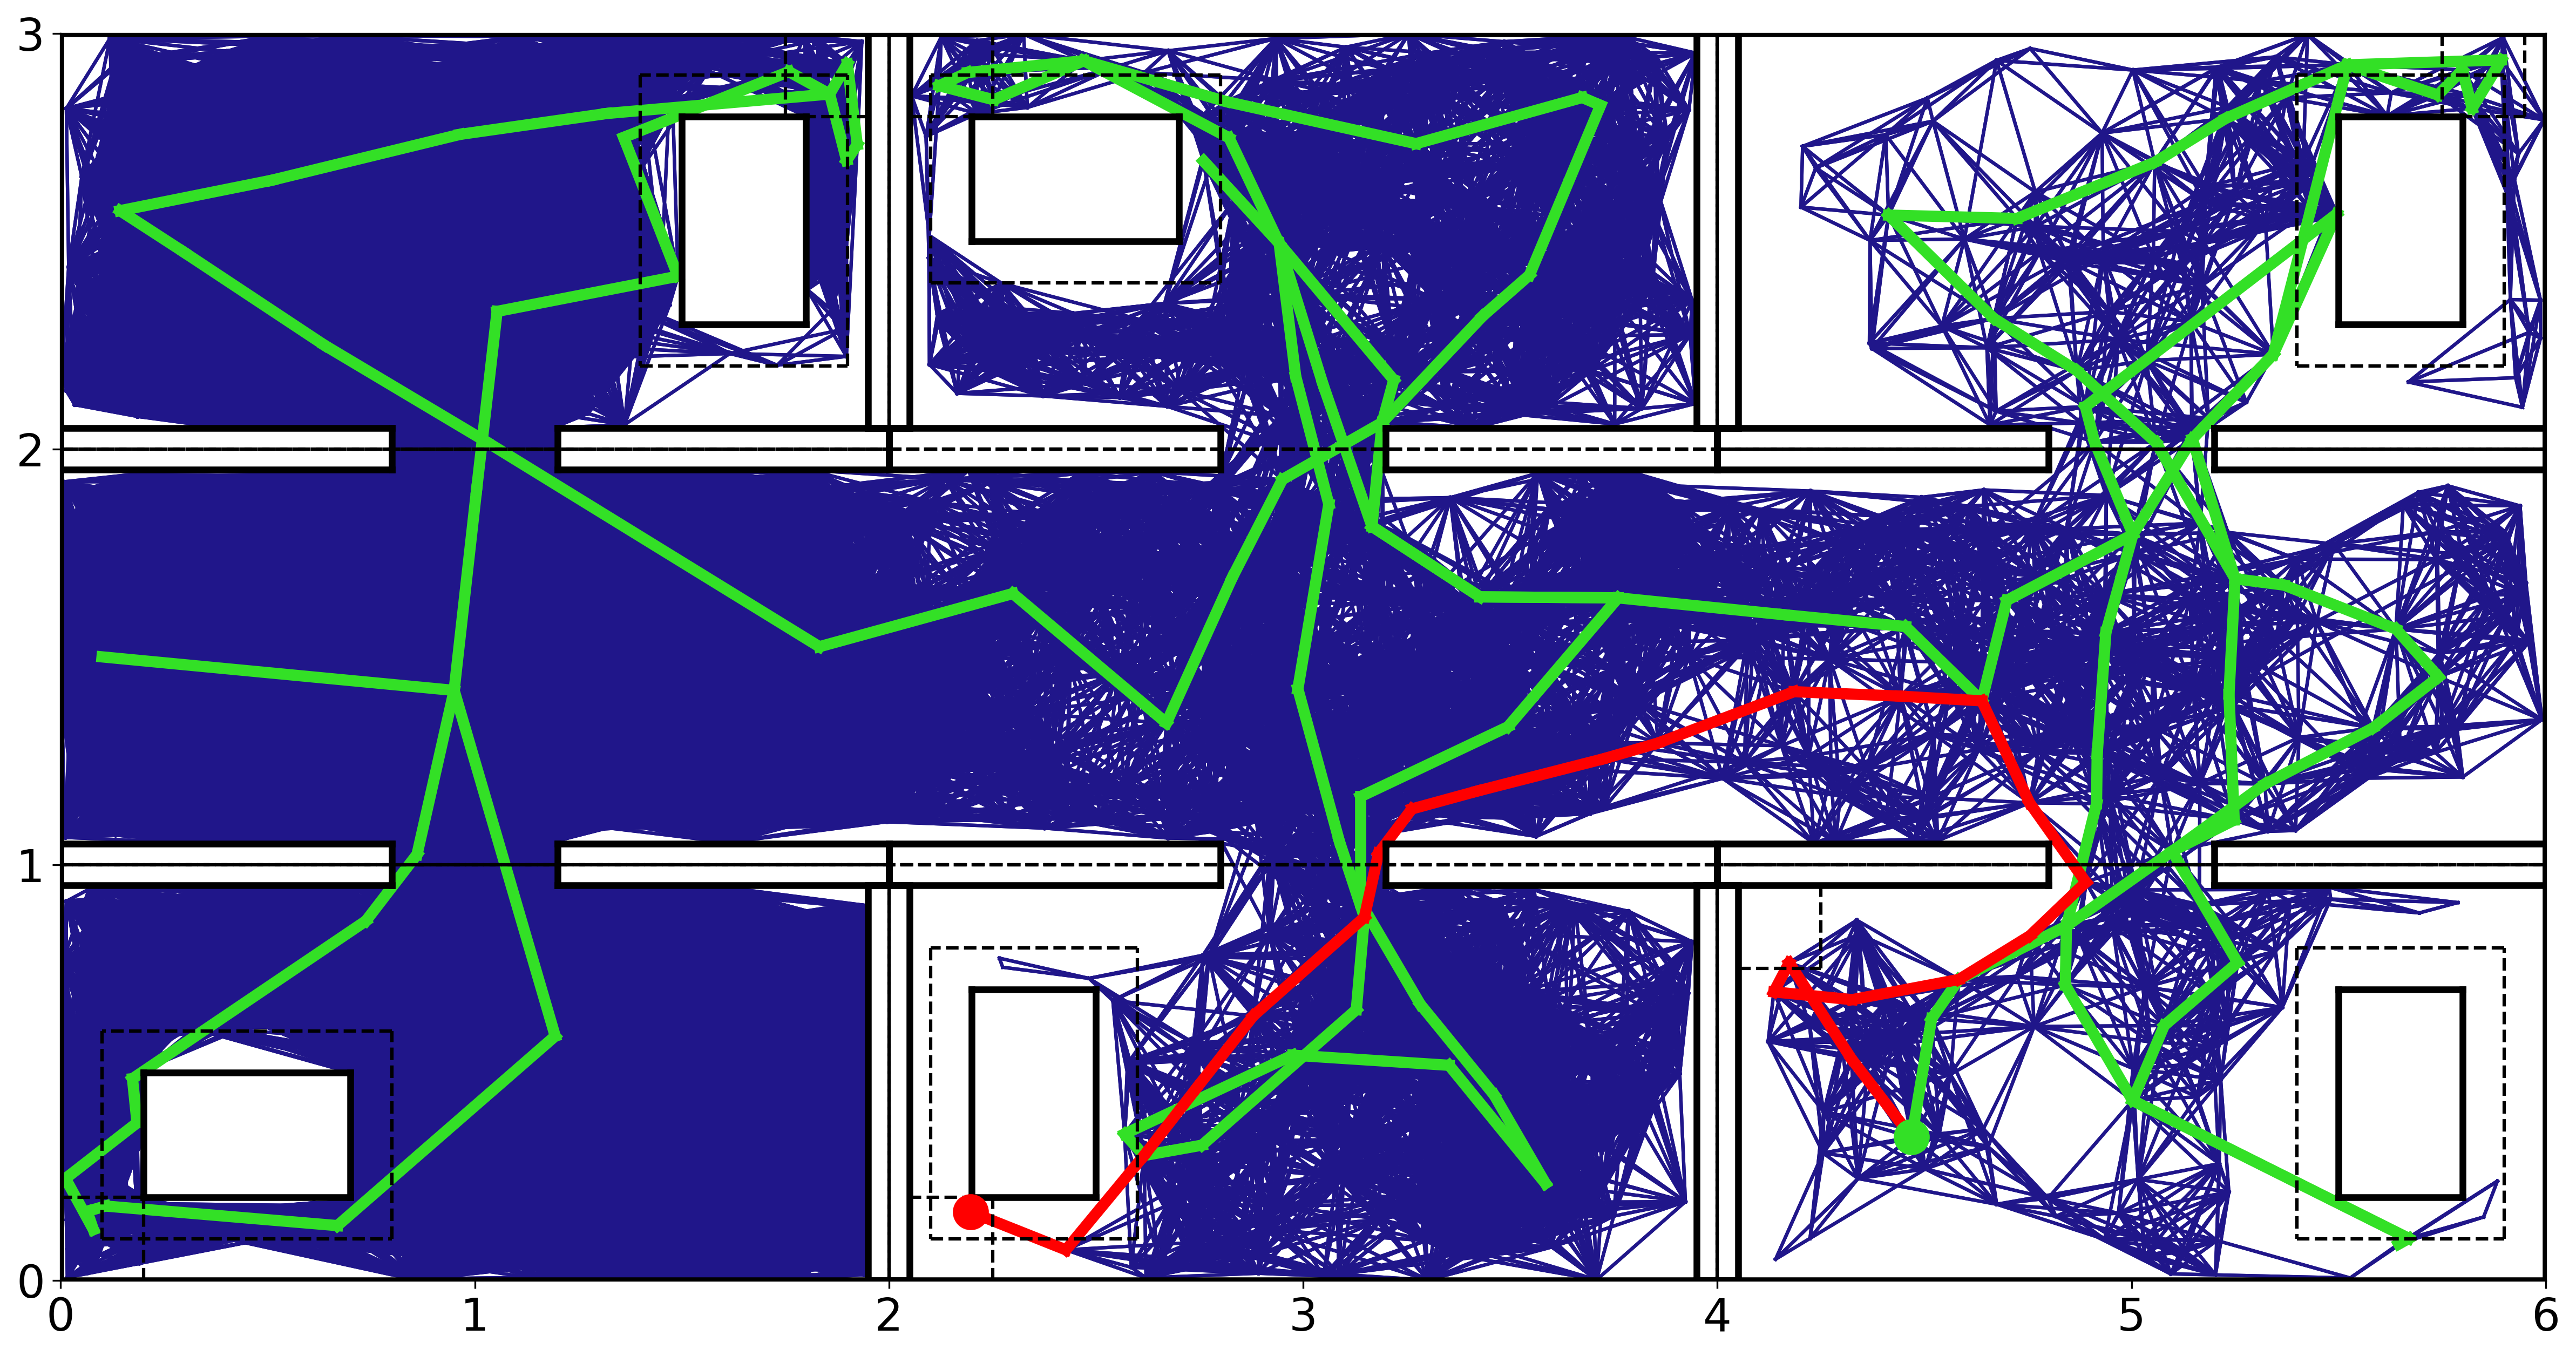
\includegraphics[width=\textwidth]{Fig/tog_final.png}
	}
\end{frame}


\begin{frame}
	\frametitle{Experiments: See Through Desks}
	Compared different approaches on 100 randomly generated office like environments.
	\vspace{15pt}
	\begin{table}%[th]
		\centering
		\scalebox{0.8}{
			\begin{tabular}{l c c c}
				\hline
				\textbf{} & \multicolumn{3}{c}{\textbf{See-through Desks}}  \\
				&\textbf{\sep}&\textbf{\tog}&\textbf{\bia}\\
				\hline
				\textbf{Total length}     & 77.3 (7.5) & 56.6 (8.0) & 29.4 (5.0) \\
				%%
				\multicolumn{1}{l}{Exploration length}  & 57.1 (3.2) & 37.5 (7.1) & 28.0 (4.9)  \\
				%\hline
				\multicolumn{1}{l}{Remaining plan l.} & 20.2 (7.0) & 19.1 (3.6) & 1.3 (1.8)\\
				%%
				\textbf{Total Time}       & 7.8 (2.0) & 6.4 (2.3) & 7.3 (1.9) \\
				%%
				\textbf{RRG size}         & 1931.2 (460.9) & 1938.6 (559.5) & 1793.6 (312.1) \\
				\hline
		\end{tabular}}
	\end{table}
\end{frame}


\begin{frame}
	\frametitle{Experiments: Opaque Desks}
	Compared different approaches on 100 randomly generated office like environments.
	\vspace{15pt}
	\begin{table}%[th]
		\centering
		\scalebox{0.8}{
			\begin{tabular}{l c c c}
				\hline
				\textbf{} & \multicolumn{3}{c}{\textbf{Opaque Desks}} \\
				&\textbf{\sep}&\textbf{\tog}&\textbf{\bia}\\
				\hline
				\textbf{Total length}    & 79.1 (7.1) & 62.9 (16.5) & 32.3 (11.8) \\
				%%
				\multicolumn{1}{l}{Exploration length} & 57.8 (4.9) & 44.4 (16.6) & 31.3 (12.1) \\
				%\hline
				\multicolumn{1}{l}{Remaining plan l.} & 21.3 (5.1) & 18.5 (3.4) & 1.1 (1.8)\\
				%%
				\textbf{Total Time}       & 9.6 (2.5) & 8.3 (3.2) & 9.1 (2.4)\\
				%%
				\textbf{RRG size}         & 2313.8 (550.9) & 1868.7 (498.2) & 1901.4 (301.2)\\
				\hline
			\end{tabular}
		}
	\end{table}
\end{frame}

\section{Conclusion and Future Work}

\begin{frame}
	\frametitle{Conclusion and Future Work}
	
	\textbf{Conclusion}
	\begin{itemize}
		\item Gave an algorithm for Motion Planning of scLTL missions in an unknown environment. \pause
		\item Use the previous experiences to help in the future. \pause
		\item Reduce the path traversed by more than 50\% compared to the naive approach.
	\end{itemize}
	\vspace{20pt}

	\textbf{What's next?}
	\begin{itemize}
		\item Can we do full LTL?. \pause
		\item Experiments on actual robots. \pause
		\item Figure out atomic propositions on-the-fly to make it work in a completely unknown environment.
	\end{itemize}
	\vspace{20pt}
	Thank You!
\end{frame}



\end{document}
